\documentclass{wissdoc}
% Autor: Roland Bless 1996-2009, bless <at> kit.edu
% ----------------------------------------------------------------
% Diplomarbeit - Hauptdokument
% ----------------------------------------------------------------
%%
%% $Id: thesis.tex 65 2012-05-10 10:32:11Z bless $
%%
% wissdoc Optionen: draft, relaxed, pdf --> siehe wissdoc.cls
% ------------------------------------------------------------------
% Weitere packages: (Dokumentation dazu durch "latex <package>.dtx")
\usepackage[numbers,sort&compress]{natbib}
%\usepackage{graphicx} 
% \usepackage{varioref}
% \usepackage{verbatim}
% \usepackage{float}    %z.B. \floatstyle{ruled}\restylefloat{figure}
% \usepackage{subfigure}
% \usepackage{fancybox} % für schattierte,ovale Boxen etc.
% \usepackage{tabularx} % automatische Spaltenbreite
% \usepackage{supertab} % mehrseitige Tabellen
% \usepackage[svnon,svnfoot]{svnver} % SVN Versionsinformation 
%% ---------------- end of usepackages -------------

%\svnversion{$Id: thesis.tex 65 2012-05-10 10:32:11Z bless $} % In case that you want to include version information in the footer

%% Informationen für die PDF-Datei
\hypersetup{
 pdfauthor={N.N.},
 pdftitle={Not set}
 pdfsubject={Not set},
 pdfkeywords={Not set}
}

% Macros, nicht unbedingt notwendig
%%%%%%%%%%%%%%%%%%%%%%%%%%%%%%%%%%%%%%%%%%%%%%%%%%%%%%%%%%
% macros.tex -- einige mehr oder weniger nuetzliche Makros
% Autor: Roland Bless 1998
%%%%%%%%%%%%%%%%%%%%%%%%%%%%%%%%%%%%%%%%%%%%%%%%%%%%%%%%%%
% $Id: macros.tex 33 2007-01-23 09:00:59Z bless $
%%%%%%%%%%%%%%%%%%%%%%%%%%%%%%%%%%%%%%%%%%%%%%%%%%%%%%%%%%


%%%%%%%%%%%%%%%%%%%%%%%
% Kommentare 
%%%%%%%%%%%%%%%%%%%%%%%
\ifnotdraftelse{
\newcommand{\Kommentar}[1]{}
}{\newcommand{\Kommentar}[1]{{\em #1}}}
% Alles innerhalb von \Hide{} oder \ignore{} 
% wird von LaTeX komplett ignoriert (wie ein Kommentar)
\newcommand{\Hide}[1]{}
\let\ignore\Hide

%%%%%%%%%%%%%%%%%%%%%%%%%
% Leere Seite ohne Seitennummer, wird aber gezaehlt
%%%%%%%%%%%%%%%%%%%%%%%%%

\newcommand{\leereseite}{% Leerseite ohne Seitennummer, n�chste Seite rechts (wenn 2-seitig)
 \clearpage{\pagestyle{empty}\cleardoublepage}
}
%%%%%%%%%%%%%%%%%%%%%%%%%%
% Flattersatz rechts und Silbentrennung, Leerraum nach rechts maximal 1cm
%%%%%%%%%%%%%%%%%%%%%%%%%%
\makeatletter
\newcommand{\myraggedright}{%
 \let\\\@centercr\@rightskip 0pt plus 1cm
 \rightskip\@rightskip
  \leftskip\z@skip
  \parindent\z@
  \spaceskip=.3333em
  \xspaceskip=.5em}
\makeatother

\makeatletter
\newcommand{\mynewline}{%
 \@centercr\@rightskip 0pt plus 1cm
}
\makeatother


%%%%%%%%%%%%%%%%%%%%%%%%%%
% F�r Index
%%%%%%%%%%%%%%%%%%%%%%%%%%
\makeatletter
\def\mydotfill{\leavevmode\xleaders\hb@xt@ .44em{\hss.\hss}\hfill\kern\z@}
\makeatother
\def\bold#1{{\bfseries #1}}
\newbox\dbox \setbox\dbox=\hbox to .4em{\hss.\hss} % dot box for leaders
\newskip\rrskipb \rrskipb=.5em plus3em % ragged right space before break
\newskip\rrskipa \rrskipa=-.17em plus -3em minus.11em % ditto, after
\newskip\rlskipa \rlskipa=0pt plus3em % ragged left space after break
\newskip\rlskipb \rlskipb=.33em plus-3em minus.11em % ragged left before break
\newskip\lskip \lskip=3.3\wd\dbox plus1fil minus.3\wd\dbox % for leaders
\newskip \lskipa \lskipa=-2.67em plus -3em minus.11em %after leaders
\mathchardef\rlpen=1000 \mathchardef\leadpen=600
\def\rrspace{\nobreak\hskip\rrskipb\penalty0\hskip\rrskipa}
\def\rlspace{\penalty\rlpen\hskip\rlskipb\vadjust{}\nobreak\hskip\rlskipa}
\let\indexbreak\rlspace
\def\raggedurl{\penalty10000 \hskip.5em plus15em \penalty0 \hskip-.17em plus-15em minus.11em}
\def\raggeditems{\nobreak\hskip\rrskipb \penalty\leadpen \hskip\rrskipa %
\vadjust{}\nobreak\leaders\copy\dbox\hskip\lskip %
\kern3em \penalty\leadpen \hskip\lskipa %
\vadjust{}\nobreak\hskip\rlskipa}
\renewcommand*\see[2]{\rlspace\emph{\seename}~#1} % from makeidx.sty

%%%%%%%%%%%%%%%%%%%%%%%%%%
% Neue Seite rechts, leere linke Seite ohne Headings
%%%%%%%%%%%%%%%%%%%%%%%%%%
\newcommand{\xcleardoublepage}
{{\pagestyle{empty}\cleardoublepage}}

%%%%%%%%%%%%%%%%%%%%%%%%%%
% Tabellenspaltentypen (benoetigt colortbl)
%%%%%%%%%%%%%%%%%%%%%%%%%%
\newcommand{\PBS}[1]{\let\temp=\\#1\let\\=\temp}
\newcolumntype{y}{>{\PBS{\raggedright\hspace{0pt}}}p{1.35cm}}
\newcolumntype{z}{>{\PBS{\raggedright\hspace{0pt}}}p{2.5cm}}
\newcolumntype{q}{>{\PBS{\raggedright\hspace{0pt}}}p{6.5cm}}
\newcolumntype{g}{>{\columncolor[gray]{0.8}}c} % Grau
\newcolumntype{G}{>{\columncolor[gray]{0.9}}c} % helleres Grau

%%%%%%%%%%%%%%%%%%%%%%%%%%
% Anf�hrungszeichen oben und unten
%%%%%%%%%%%%%%%%%%%%%%%%%%
\newcommand{\anf}[1]{"`{#1}"'}

%%%%%%%%%%%%%%%%%%%%%%%%%%
% Tiefstellen von Text
%%%%%%%%%%%%%%%%%%%%%%%%%%
% S\tl{0} setzt die 0 unter das S (ohne Mathemodus!)
% zum Hochstellen gibt es uebrigens \textsuperscript
\makeatletter
\DeclareRobustCommand*\textlowerscript[1]{%
  \@textlowerscript{\selectfont#1}}
\def\@textlowerscript#1{%
  {\m@th\ensuremath{_{\mbox{\fontsize\sf@size\z@#1}}}}}
\let\tl\textlowerscript
\let\ts\textsuperscript
\makeatother

%%%%%%%%%%%%%%%%%%%%%%%%%%
% Gau�-Klammern
%%%%%%%%%%%%%%%%%%%%%%%%%%
\newcommand{\ceil}[1]{\lceil{#1}\rceil}
\newcommand{\floor}[1]{\lfloor{#1}\rfloor}

%%%%%%%%%%%%%%%%%%%%%%%%%%
% Average Operator (analog zu min, max)
%%%%%%%%%%%%%%%%%%%%%%%%%%
\def\avg{\mathop{\mathgroup\symoperators avg}}

%%%%%%%%%%%%%%%%%%%%%%%%%%
% Wortabk�rzungen
%%%%%%%%%%%%%%%%%%%%%%%%%%
\def\zB{z.\,B.\ }
\def\dh{d.\,h.\ }
\def\ua{u.\,a.\ }
\def\su{s.\,u.\ }
\newcommand{\bzw}{bzw.\ }

%%%%%%%%%%%%%%%%%%%%%%%%%%%%%%%%%%%
% Einbinden von Graphiken
%%%%%%%%%%%%%%%%%%%%%%%%%%%%%%%%%%%
% global scaling factor
\def\gsf{0.9}
%% Graphik, 
%% 3 Argumente: Datei, Label, Unterschrift
\newcommand{\Abbildung}[3]{%
\begin{figure}[tbh] %
\centerline{\scalebox{\gsf}{\includegraphics*{#1}}} %
\caption{#3} %
\label{#2} %
\end{figure} %
}
\let\Abb\Abbildung
%% Abbps
%% Graphik, skaliert, Angabe der Position
%% 5 Argumente: Position, Breite (0 bis 1.0), Datei, Label, Unterschrift
\newcommand{\Abbildungps}[5]{%
\begin{figure}[#1]%
\begin{center}
\scalebox{\gsf}{\includegraphics*[width=#2\textwidth]{#3}}%
\caption{#5}%
\label{#4}%
\end{center}
\end{figure}%
}
\let\Abbps\Abbildungps
%% Graphik, Angabe der Position, frei w�hlbares Argument f�r includegraphics
%% 5 Argumente: Position, Optionen, Datei, Label, Unterschrift
\newcommand{\Abbildungpf}[5]{%
\begin{figure}[#1]%
\begin{center}
\scalebox{\gsf}{\includegraphics*[#2]{#3}}%
\caption{#5}%
\label{#4}%
\end{center}
\end{figure}%
}
\let\Abbpf\Abbildungpf

%%
% Anmerkung: \resizebox{x}{y}{box} skaliert die box auf Breite x und H�he y,
%            ist x oder y ein !, dann wird das uspr�ngliche 
%            Seitenverh�ltnis beibehalten.
%            \rescalebox funktioniert �hnlich, nur das dort ein Faktor
%            statt einer Dimension angegeben wird.
%%
% \Abbps{Position}{Breite in Bruchteilen der Textbreite}{Dateiname}{Label}{Bildunterschrift}
%

\newcommand{\refAbb}[1]{%
s.~Abbildung \ref{#1}}

%%%%%%%%%%%%%%%%%%%%
%% end of macros.tex
%%%%%%%%%%%%%%%%%%%%

% Print URLs not in Typewriter Font
\def\UrlFont{\rm}

\newcommand{\blankpage}{% Leerseite ohne Seitennummer, nächste Seite rechts
 \clearpage{\pagestyle{empty}\cleardoublepage}
}

%% Einstellungen für das gesamte Dokument

% Trennhilfen
% Wichtig! 
% Im ngerman-paket sind zusätzlich folgende Trennhinweise enthalten:
% "- = zusätzliche Trennstelle
% "| = Vermeidung von Ligaturen und mögliche Trennung (bsp: Schaf"|fell)
% "~ = Bindestrich an dem keine Trennung erlaubt ist (bsp: bergauf und "~ab)
% "= = Bindestrich bei dem Worte vor und dahinter getrennt werden dürfen
% "" = Trennstelle ohne Erzeugung eines Trennstrichs (bsp: und/""oder)

% Trennhinweise fuer Woerter hier beschreiben
\hyphenation{
% Pro-to-koll-in-stan-zen
% Ma-na-ge-ment  Netz-werk-ele-men-ten
% Netz-werk Netz-werk-re-ser-vie-rung
% Netz-werk-adap-ter Fein-ju-stier-ung
% Da-ten-strom-spe-zi-fi-ka-tion Pa-ket-rumpf
% Kon-troll-in-stanz
}

% Index-Datei öffnen
\ifnotdraft{\makeindex}
%%%%%%%%%%%%%% includeonly %%%%%%%%%%%%%%%%%%%
% Es werden nur die Teile eingebunden, die hier 
% aufgefuehrt sind!
\includeonly{%
titelseite,%
erklaerung,% Ist in KA Pflicht für Diplomarbeiten
einleitung,% Motivation, Zielsetzung, Gliederung
vorherige,
grundlagen,% Grundlagen 
analyse,   % Problembeschreibung (Detail) und Related Work
entwurf,   % Beschreibung der Problemlösung (Konzepte, allg. Architektur, ...)
implemen,  % Beschreibung der Umsetzung/Implementierung
eval,      % Nachweis und Auswertung
zusammenf  % Zusammenfassung der Ergebnisse und Ausblick
}
%%%%%%%%%%%%%%%%%%%%%%%%%%%%%%%%%%%%%%%%%%%%%%
\begin{document}

\frontmatter
\pagenumbering{roman}
\ifnotdraft{
 %% Titelseite
%% Vorlage $Id: titelseite.tex 61 2012-05-03 13:58:03Z bless $

\def\usesf{}
\let\usesf\sffamily % diese Zeile auskommentieren für normalen TeX Font

\newsavebox{\Erstgutachter}
\savebox{\Erstgutachter}{\usesf Prof.~Dr.~H.~Schmeck}
\newsavebox{\Zweitgutachter}
\savebox{\Zweitgutachter}{\usesf Prof.~Dr.~?.~?????????}

\begin{titlepage}
\setlength{\unitlength}{1pt}
\begin{picture}(0,0)(85,770)

\includegraphics[width=\paperwidth]{logos/KIT_Deckblatt}
\end{picture}

\thispagestyle{empty}

%\begin{titlepage}
%%\let\footnotesize\small \let\footnoterule\relax
\begin{center}
\hbox{}
\vfill
{\usesf
{\huge\bfseries Energieoptimierung WLAN-basierter Ortungseinheiten \par}
\vskip 1.8cm
Masterarbeit\\
von\\[2mm]
\vskip 1cm

{\large\bfseries Marius Wodtke\\}
\vskip 1.2cm
Institut für Angewandte Informatik und Formale Beschreibungsverfahren (AIFB)\\
der Fakultät für Informatik\\
%Universität Karlsruhe (TH)\\[2ex]
\vskip 3cm
\begin{tabular}{p{5.5cm}l}
Erstgutachter: & \usebox{\Erstgutachter} \\
Zweitgutachter: & \usebox{\Zweitgutachter} \\
Betreuender~Mitarbeiter: & Dipl.-Inform.~K.~Bao \\
\end{tabular}
\vskip 3cm
Bearbeitungszeit:\qquad 01.~April~2017 -- 31.~Oktober~2017
}
\end{center}
\vfill
\end{titlepage}
%% Titelseite Ende


%%% Local Variables: 
%%% mode: latex
%%% TeX-master: "thesis"
%%% End: 

 \blankpage % Leerseite auf Titelrückseite
 %
 % Die folgende Erklärung ist für Diplomarbeiten Pflicht
 % (siehe Prüfungsordnung), für Studienarbeiten nicht notwendig
 \thispagestyle{empty}
\vspace*{32\baselineskip}
\hbox to \textwidth{\hrulefill}
\par
Ich erkl�re hiermit, dass ich die vorliegende Arbeit selbst�ndig verfasst und
keine anderen als die angegebenen Quellen und Hilfsmittel benutzt, 
die w�rtlich oder inhaltlich �bernommenen Stellen als solche kenntlich 
gemacht und die Satzung des KIT zur Sicherung guter wissenschaftlicher 
Praxis in der jeweils g�ltigen Fassung beachtet habe.

\vspace*{2cm}
Karlsruhe, den ??. ?????? 201?\hfill \hbox to 8cm{\hrulefill}

%%%%%%%%%%%%%%%%%%%%%%%%%%%%%%%%%%%%%%%%%%%%%%%%%%%%%%%%%%%%%%%%%%%%%%%%
%% Hinweis:
%%
%% Diese Erkl�rung wird von der Pr�fungsordnung f�r Diplom-, Master,
%% und Bachelorarbeiten verlangt und ist zu unterschreiben. 
%% F�r Studienarbeiten ist diese Erkl�rung nicht zwingend notwendig, 
%% schadet aber auch nicht.
%%%%%%%%%%%%%%%%%%%%%%%%%%%%%%%%%%%%%%%%%%%%%%%%%%%%%%%%%%%%%%%%%%%%%%%%
\clearpage







 \blankpage % Leerseite auf Erklärungsrückseite
}
%
%% *************** Hier geht's ab ****************
%% ++++++++++++++++++++++++++++++++++++++++++
%% Verzeichnisse
%% ++++++++++++++++++++++++++++++++++++++++++
\ifnotdraft{
{\parskip 0pt\tableofcontents} % toc bitte einzeilig
\blankpage
%\listoffigures
%\blankpage
%\listoftables
%\blankpage
}


%% ++++++++++++++++++++++++++++++++++++++++++
%% Hauptteil
%% ++++++++++++++++++++++++++++++++++++++++++
\graphicspath{{Bilder/}}

\mainmatter
\pagenumbering{arabic}
\chapter{Einleitung}
\label{ch:Einleitung}
Während die Ortung im Außenbereich fest in der Hand von Satellitennavigationssystemen wie dem Global Positioning System (GPS) liegen, existiert für die Ortung im Innenraum eine Vielzahl verschiedener Technologien. Neben Technologien wie Bluetooth, Radio Frequency Identification (RFID) und Ultra Wide Band (UWB) weckt WLAN wegen seiner großen Verbreitung immer wieder Interesse in Forschung und Industrie. 

So hat die Ortung mittels WLAN gerade im medizinischen Bereich durch kommerzielle Lösungen Verbreitung gefunden, Probleme finden sich aber bei Ortungsgenauigkeit gegenüber anderen Techniken und dem vergleichsweise hohen Energieverbrauch des WLAN-Protokolls.
Während sich viele wissenschaftliche Arbeiten der Ortungsgenauigkeit widmen, ist für den alltäglichen Einsatz die kurze Batterielaufzeit der mobilen Einheiten hinderlich, wenn nicht zum Beispiel Smartphones als mobile Einheiten in Frage kommen. 

Auch im Tunnelbau ist eine Ortung von Mitarbeitern und Besuchern von Nöten um in Notfällen bestimmen zu können, ob und wie viele Personen sich im Gefahrenbereich befinden. 
Dies beeinflusst die Arbeit der Rettungskräfte. 
Das veränderliche Umfeld der Baustelle, auf der große Stahl- und Betonelemente bewegt werden, stellt dabei die genaue Ortung mittels Radiowellen vor große Probleme und es wird nur eine Bereichsortung durchgeführt, bei der jede Tunnelröhre in mehrere hundert Meter große Abschnitte aufgeteilt wird und der Wechsel der Mitarbeiter zwischen den Abschnitten beobachtet wird. 
Dies stellt zwar nur eine geringe Genauigkeit dar, erlaubt es aber bei Bränden zu erkennen, welche Personen sich durch die Abschnitte Richtung Ausgang bewegen und welche in ihrem Abschnitt verharren. 
Solche Personen sind vermutlich bewegungsunfähig oder eingeschlossen.


\section{Bisherige Situation}
Die Ortung wird derzeit bei der Ed. Züblin AG mittels Bluetooth durchgeführt. 
Dabei sind die Basisstationen eigenständige Bluetooth-Einheiten, die mit dem Ethernet Backbone verbunden sind.
Als mobile Einheiten kommen sowohl batteriebetriebene "`Tags"' als auch Smartphones zum Einsatz. 
Das zentrale Sicherheitssystem fragt die gesehenen mobilen Einheiten bei den Basisstationen an und bereitet die Ergebnisse graphisch auf.

Der Tunnel wird in Bereiche zu circa 500 Meter aufgeteilt, die Tunnelbohrmaschine (TBM) stellt dabei einen Sonderbereich dar, weil sie sich im Gegensatz zu den anderen Bereichen langsam bewegt. 
Neue Bereiche werden hinter der TBM eingefügt und sind dann stationär.

Die Bluetooth-Basisstationen werden in Kästen verstaut, die weitere notwendige Technik, wie etwa ein Notfalltelefon, enthalten.
Weil diese Kästen nur etwa alle 500 Meter montiert sind, existieren große Lücken in denen die mobilen Einheiten nicht geortet werden.
Eine mobile Einheit wird im System so lange im selben Bereich angezeigt, bis sie wieder von einer Basisstation erkannt wird.

Wird die mobile Einheit von der Erfassungseinheit vor dem Portal (Tunneleingang) erkannt gilt sie als außerhalb des Tunnels.
Abbildung \ref{fig:bisherige} zeigt die bisherige Situation mit Bluetooth-Basisstaionen. 
Die Reichweite der der Basistationen ist dabei nicht maßstabsgetreu.

\begin{figure}[h]
  \centering
	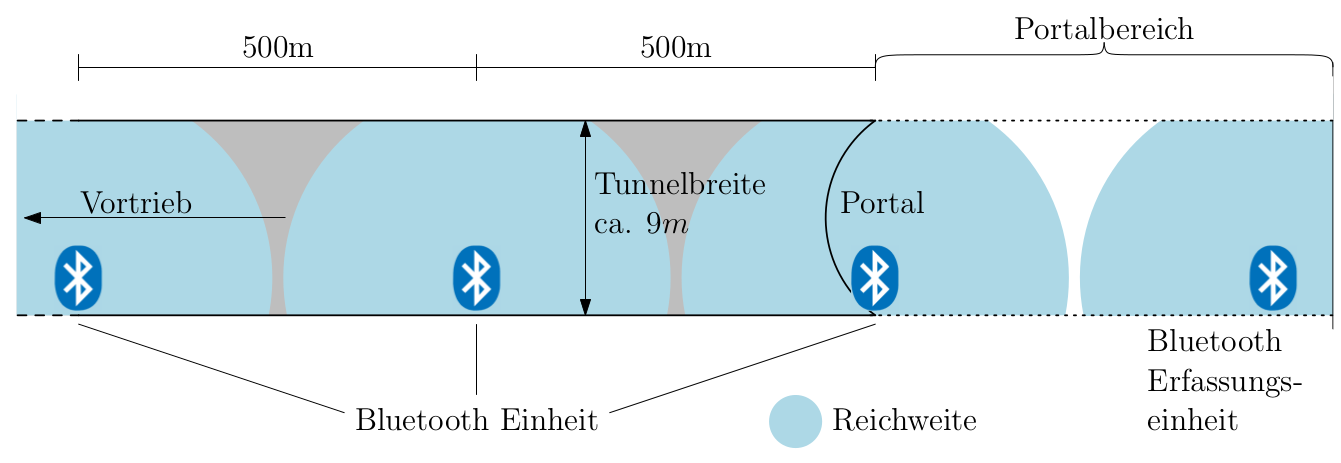
\includegraphics[width=\textwidth]{images/bisherige.png}
  \caption{Bereichsortung mit Bluetooth, aus \cite{maurer2016unterstuetzung}.}
  \label{fig:bisherige}
\end{figure}

 
\section{Umgebung für funkbasierte Ortung}
Als Versuchsumgebung dient die Tunnelbaustelle Rastatt.
Dort gelten die Positionen der Kästen für die Technik als unveränderlich.
Nur sie bieten Strom, Netzwerkanbindung (LAN) und Schutz vor dem Baustellenumfeld.
Für Funkprotokolle, die weniger als 250 Meter Reichweite entfalten muss daher mit Erfasssungslücken gerechnet werden.
Auf der TBM und anderen technischen Fahrzeugen sind jedoch mehr Basisstationen möglich.

Es existiert bereits ein WLAN-Netzwerk, dessen Access Points als Basisstationen genutzt werden können.
Es handelt sich um APs der Firma Lancom, diese stellt auch ein Modell LN-862 für Versuche.
Für zukünftige Baustellen soll der Abstand der Versorgungskästen auf 250 Meter sinken. 
Diese Situation ist in Abbildung \ref{fig:zukuenftige} skizziert.

\begin{figure}[h]
  \centering
	\includegraphics[width=\textwidth]{images/zukuenftige.eps}
  \caption{Zukünftige Situation der Tunnelbaustellen.}
  \label{fig:zukuenftige}
\end{figure}

\section{Problemstellung}
Es muss ein System geschaffen werden, welches Mitarbeiter einem 250 Meter langen Abschnitt innerhalb eines im Bau befindlichen Tunnels zuordnet.
Dazu soll keine Nutzerinteraktion nötig sein, der Nutzer wird wird über eine mobile Einheit geortet.
Die Ortung muss unterirdisch funktionieren und robust gegenüber Stahlhindernissen sein.
Außerdem können Basisstation für die Ortung nur alle 250 Meter platziert werden.


\section{Zielsetzung der Arbeit}
\label{ch:Einleitung:sec:Zielsetzung}
Ziel der Arbeit soll der Entwurf und die Implementierung eines Bereichsortungssystems für Personen in Tunnelanlagen sein. 
Bei einem Bereichsortungssystem handelt es sich um ein Ortungssystem, bei dem die Positionen nicht genau bestimmt werden. 
Stattdessen wird das Areal, auf dem geortet werden soll, in einzelne Bereiche unterteilt und jede mobile Einheit beim Vorgang des Ortens einem dieser Bereiche zugeordnet.

Diese Arbeit grenzt sich von vorherigen Arbeiten dadurch ab, dass die Laufzeit beziehungsweise der Energieverbrauch der mobilen Einheiten im Vordergrund steht. 
Ziel dieser Arbeit ist eine mehrmonatige Laufzeit der mobilen Einheiten. 

Für diese Arbeit werden mehrere Prototypen für mobile Einheiten entwickelt und auf ihre Charakteristik bezüglich des Energieverbrauchs und der Erkennungszuverlässigkeit untersucht.
Der Entwurfsraum umfasst dabei die Hardware und Software der mobilen Enheit sowie die Implementierung des Ortungsdienstes. 
Die für die Funktechnologie benötigte Infrastruktur wird jeweils als gegeben angenommen.


\section{Anforderungen an das Bereichsortungssystem}
\label{ch:Einleitung:sec:Anforderungen}
Da es sich um ein Bereichsortungssystem handeln soll, werden keine direkten Anforderungen an die Genauigkeit der Ortung gestellt. 
Jedoch soll ein klarer Wechsel zwischen zwei Bereichen, und damit zwei Basisstationen, zuverlässig erkannt werden. 
Die mobilen Einheiten sollen von Personen um den Hals getragen werden können. 
Dies bedingt ein geringes Gewicht des Akkus, gleichzeitig soll aber die Laufzeit der mobilen Einheit maximiert werden, sodass ein Akku mit möglichst großer Kapazität gewählt werden sollte.
Zuletzt soll unter Rücksichtnahme auf das beschriebene Szenario die Komplexität der benötigten IT-Infrastruktur so gering wie möglich gehalten werden um ein stabiles und kostengünstiges System zu garantieren. 


\section{Gliederung der Arbeit}
\label{ch:Einleitung:sec:Gliederung}
Nachdem zunächst in Kapitel \ref{ch:Grundlagen} die Grundlagen der funkbasierten Ortung und der verwendeten Funkprotokolle behandelt werden, wird in Kapitel \ref{ch:Analyse} das Problem analysiert und verwandte Arbeiten aufgezeigt.
Kapitel \ref{ch:Implementierung} beschäftigt sich mit der Implementierung und Untersuchung der Prototypen. 
Das Fazit in Kapitel \ref{ch:Fazit} fasst die Arbeit noch einmal zusammen, vergleicht und bewertet die Ergebnisse.
  % Einleitung
%TODO Bluetooth Beispiel

\chapter{Vorherige Arbeiten}
\label{ch:Vorherige}
%% ==============================
In diesem Kapitel werden vorhandene Lösungen, die für die gegebene Aufgabe der Bereichsortung in Tunneln in Frage kommen, diskutiert. 
Es werden hauptsächlich Lösungen auf Basis der 802.11 Spezifikation ausgewählt, dabei aber auch solche Systeme einbezogen, die eine spezifische Position der mobilen Einheit angeben, da diese anschließend trivial einem Bereich zugeordnet werden kann. 
Es werden sowohl wissenschaftliche als auch kommerzielle Lösungen diskutiert.\\
Auffällig ist bei der Recherche, dass wissenschaftliche Veröffentlichungen sich fast immer auf eines von zwei Aufgabenfeldern beziehen: Entweder soll die Ortungsgenauigkeit erhöht oder die Anforderungen ohne signifikanten Genauigkeitsverlust gesenkt werden. 
Diese Anforderungen können zum Beispiel Komplexität des Knoten-Netzwerks, des einzelnen Knotens, Synchronisation oder vorherige Kalibrierung sein.\\
An den Energieverbrauch der mobilen Einheiten werden üblicherweise keine Forderungen gestellt und oft von den Veröffentlichungen komplett ignoriert.
Dies ist akzeptabel wenn davon ausgegangen wird, dass die mobile Einheit zusätzlichen Nutzen bietet und das Laden der Einheit in Nutzungsszenario des Anwenders bereits vorgesehen ist.
So hat der Anwender in einem Szenario, bei dem sein Smartphone mittels direkter oder indirekter Selbstlokalisierung seine Position bestimmt um ihn zu navigieren nur minimale Anforderungen an den Energieverbrauch.
In Szenarien mit direkter oder indirekter Fernlokalisierung hat die mobile Einheit für den Anwender oft keinen direkten Nutzen, deshalb ist eine Forderung nach täglichem oder wöchentlichem Laden beziehungsweise Wechseln der Batterie schwerer durchzusetzen.\\





\subsection{Ultraschall}
Skibiniewski et al. nutzen Ultraschall für eine Fernlokalisierung mit TOF \cite{skibniewski2009simulation}.
Ultraschall kann nicht von WLAN APs empfangen werden und es muss zusätzliche Hardware installiert werden, das System soll hier dennoch Beachtung finden, da es für die Ortung von Baumaterial auf Baustellen entwickelt wurde.\\
Bei diesem System sendet zunächst der Knoten einen Beacon Frame der ZigBee Spezifikation (802.15.4) an die mobile Einheit, diese antwortet und sendet unmittelbar danach das Ultraschallsignal.
Das schnelle 2.4GHz ZigBee Signal dient dem Knoten dann als Referenz für den Sendezeitpunkt des Ultraschallsignals, welches wegen seiner langsamen Ausbreitungsgeschwindigkeit $c \approx 343m/s$ wesentlich weniger anfällig für ungenaue Zeitstempel ist. 
Außerdem kann die Zeit zwischen dem Aussenden des Beacon Frames und der Antwort gemessen werden um zusätzliche TOF-Informationen zu gewinnen. \\
Statt ZigBee ließe sich auch WLAN nutzen, ZigBee ist jedoch bereits auf niedrigen Energieverbrauch ausgelegt und wegen des Ultraschalls wäre trotzdem ein extra Knoten nötig.
Problematisch an der Lösung ist entweder der Energieverbrauch der Ultraschalleinheit oder die Reichweite, ausreichend kleine Einheiten reichen keine 100m weit und leiden trotzdem unter kurzer Batterielaufzeit.
Die Autoren schließen deshalb, dass noch Innovation in diesem Bereich notwendig ist um dieses System praktikabel zu machen.

\section{LANDMARC}
\label{ch:Vorherige:sec:LANDMARC}
Ni et al. stellen ein Ortungssystem auf Basis von Radio Frequency Identification (RFID) vor \cite{ni2004landmarc}.
Dazu werden aktive RFID-Tags als mobile Einheiten eingesetzt, diese sind mit einer Batterie ausgestattet und senden regelmäßig ihre gespeicherte ID aus.\\
Der Knoten ist mit einem Lesegerät (RFID-Reader) ausgestattet und empfängt die ID, der Knoten liefert dann die ID und ein Signalstärkelevel zwischen 1 und 8 zurück. 
Da das Signalstärkelevel nur eine sehr grobe Auflösung hat verbessern Ni et al. die Genauigkeit durch das Ausbringen von zusätzlichen Tags an bekannten, fixen Positionen, für die Bereichsortung ist dies aber nicht notwendig.\\
Die Autoren geben für ein Sendeintervall von 7,5 Sekunden eine Batterielaufzeit von 3-5 Jahren an, dabei sind die Tags klein genug und könnten, wie in der Einleitung gefordert, an einem Band um den Hals getragen werden.
%"System lässt sich leicht auf Bluetooth übertragen"

\section{Bluetooth}
\label{ch:Vorherige:sec:Bluetooth}
Hier habe ich noch kein Paper, es kommt aber fix noch mindestens ein System auf Bluetooth-Basis + Kritik an verschiedenen Buetooth Parametern.



\chapter{Analyse}
\label{ch:Analyse}
In diesem Kapitel werden zunächst einige verwandte Arbeiten vorgestellt und danach werden auf Basis dieser die Topologie, Protokolle und Messwerte für die Implementierungen dieser Arbeit ausgewählt.

\section{Verwandte Arbeiten} 
Die verwandten Arbeiten wurden in drei Unterkategorien unterteilt. 
Die erste Kategorie beschäftigt sich mit Selbstlokalisierung beziehungsweise indirekter Fernlokalisierung mittels 802.11.
Die Arbeiten der zweiten Kategorie basieren ebenfalls auf 802.11, hier wird jedoch eine Fernlokalisierung oder eine indirekte Selbstlokalisierung durchgeführt.
Die letzte Kategorie beschäftigt sich mit Arbeiten, die nicht auf 802.11 basieren, hier sind Verfahren beschrieben, die andere Protokolle verwenden.

\subsection{Verwandte Arbeiten - Selbstlokalisierung \& indirekte Fernlokalisierung mit 802.11}
Für die Selbstlokalisierung mit 802.11 werden auf der mobilen Einheit Messwerte für empfangene Pakete bestimmt und daraus die Position der mobilen Einheit berechnet.
Diese Information kann anschließend an einen Ortungsserver übertragen werden, dann handelt es sich um eine indirekte Fernlokaliserung.

\subsubsection{WiFi-LLS}
\label{ch:Vorherige:sec:LLS}
Chen et al. stellen mit dem WiFi-based Local Location System (WiFi-LLS) ein System zur indirekten Fernlokalisierung vor \cite{chen2007design}.
Als Messgröße wird die Stärke des empfangenen Signals (received signal strength, RSS) genutzt. 
Diese wird laut 802.11 Spezifikation als Index (RSSI) von der Hardware zurückgegeben. \\
Für die Ortung wird zunächst der RSSI von Paketen naher Access Points gemessen und zusammen mit der MAC-Adresse der mobilen Einheit in ein Paket gepackt und an den Ortungsserver versendet.
Anschließend wird auf dem Ortungsserver ein theoretisches Signalausbreitungsmodell $P(d) = P(d_0) - 10log_{10}(\frac{d}{d_0})^n - OAF$ mit der Distanz $d$, der Signalstärke $P(d)$ und der Referenzdistanz $d_0 = 1$m zur Bestimmung der Position der mobilen Einheit verwendet. \\
$P(d_0)$, der Pfadverlustexponent $n$ und der Hindernisdämpfungsfaktor $OAF$ müssen bestimmt werden, jedoch lassen sich $P(d_0)$ und $n$ auf einer einzelnen Teststrecke mit unterschiedlichen Abständen von AP und mobiler Einheit bestimmen. $OAF$ kann sogar für einen Gebäudetyp einmalig bestimmt werden.
Dadurch hat das Modell einen konstanten Aufwand. 
Dies ist für Baustellen interessant, da sich diese Werte einmalig messen und dann sogar über mehrere gleichartige Baustellen übertragen ließen.\\
In dieser Veröffentlichung steht die Ortungsgenauigkeit im Vordergrund und es werden keine Angaben zum Energieverbrauch gemacht. 
Als Referenz kann dienen, dass die mobile Einheit bei WiFi-LLS alle 5 Sekunden einen Scan (siehe Abschnitt \ref{ch:phase1:sec:scan}) durchführt, dann werden die Signalstärken entdeckter APs zusammen mit der eigenen MAC-Adresse in XML codiert und das so erzeugte Paket an den Ortungsserver versendet.

\subsubsection{AiRISTA Flow RTLS}
Ekahau bietet unter der Marke \textit{AiRISTA Flow RTLS} eine zu WiFi-LLS ähnliche Lösung kommerziell an \cite{airista2017airista}.
Ihr Ekahau B4 Badge Tag ermittelt regelmäßig den RSSI zu nahegelegenen APs und versendet diese an einen Ortungsserver \cite{liu2007survey}.
Das Tag bietet darüber hinaus noch einige Zusatzfunktionen, so können über die Datenverbindung auch Nachrichten und Alarmierungen an das Tag gesendet werden und die drei angebrachten Knöpfe können programmiert werden.\\
Bezüglich des Energieverbrauchs gibt sich das Informationsblatt des B4 Badge Tag vage: Das Tag soll abhängig vom Ortungsintervall wochenlang halten, danach muss der $600\ mA/h$ Akku geladen werden \cite{ekahau2017b4}.
Das Informationsblatt zum Ekahau W4, welches statt um den Hals am Handgelenk getragen wird, gibt an, dass der verbaute $530\ mA/h$ Akku bei einem Ortungsintervall von 15 Sekunden 500 Stunden (ca. 21 Tage) hält \cite{ekahau2017w4}.\\
AiRISTA Flow spricht auf ihrer Website zum Beispiel Krankenhäuser, Schulen und Regierungseinrichtungen an, hier sollen zusätzlich bewegliche Objekte, wie etwa Krankenhausbetten, geortet werden.
Die dazu verwendeten Asset Tags werden über einen Beschleunigungssensor aktiviert und können, wenn die Objekte selten bewegt werden, deutlich längere Laufzeiten erreichen \cite{ekahau2017a4}. \\
Im Umfeld des Tunnelbaus zeigte sich jedoch, dass die Tags keinesfalls wochenlange Laufzeiten aufwiesen, stattdessen entluden sie sich teilweise in unter zwölf Stunden.

\subsubsection{AeroScout}
Auch das AeroScout System von Stanley Healthcare richtet sich an den medizinischen Sektor und soll Objekte und Personen orten \cite{aeroscout2017asset}, \cite{aeroscout2017staff}.
Da sich auch dieses System in das bestehende WLAN-Netzwerk einfügt, sollte es ebenfalls auf einer indirekten Fernlokalisierung beruhen und demnach ähnliche Eigenschaften bezüglich des Energieverbrauchs aufweisen.\\
Das Informationsblatt ihres T14 Tags für Personen gibt eine Laufzeit von bis zu drei Wochen, abhängig von Konfiguration und Typ des Tags, an \cite{aeroscout2017t14}. 
Eine Angabe zu dem verwendeten Typ, der Konfiguration oder der Kapazität des verbauten Akkus wird nicht gemacht.\\

\subsubsection{Selbstlokalisierung mit Szenenanalyse}
\label{ch:Vorherige:sec:RSS-basierte}
Prasithsangaree et al. stellen ein System zur Selbstlokalisierung vor \cite{prasithsangaree2002indoor}, es verwendet aber eine offline-Phase zum Sammeln von Fingerabdrücken für Positionen in einem Abstand von 1,5 beziehungsweise 3 Metern. 
In diesen Fingerabdrücken werden die gemessenen RSSI der von den APs empfangenen Pakete als Merkmale zusammen mit der Position als Label gespeichert.
In der anschließenden online-Phase werden die gemessenen RSSI mit den Fingerabdrücken verglichen und die Position als gewichtetes Mittel der Labels bestimmt. \\
Die offline-Phase ist natürlich im Sinne der Aufgabenstellung nicht sinnvoll, da für eine Tunnelbreite von im Schnitt zehn Metern 4000 beziehungsweise 2000 Messungen pro Kilometer vorgenommen werden müssten.
Generell eignen sich Lösungen mit Szenenanalyse nicht gut für Baustellen, da diese nicht auf die potentiell höhere Genauigkeit angewiesen sind. 
Üblicherweise müssen dort sehr große Flächen vermessen werden und die Veränderungen durch den Baufortschritt führen dazu, dass regelmäßig neu gemessen werden muss.
Außerdem müssen bewegliche Störquellen wie Baumaschinen vorher aus dem Bereich entfernt werden, um unverfälschte Fingerabdrücke zu erhalten.
Der Aufwand ein System mit Szenenanalyse auf einer Baustelle zu betreiben ist deshalb sehr hoch und widerspricht der Forderung nach geringer Komplexität. \\
Die Arbeit zeigt aber die Volatilität der empfangenen Signalstärke auf, dies wurde 2011 von Lui et al. genauer untersucht \cite{lui2011differences}.
Lui et al. zeigen, dass die gemessene empfangene Signalstärke stark von der beteiligten Hardware abhängt und die Systeme jedes mal neu kalibriert werden müssen wenn sie auf ein neues AP-Modell portiert werden. 
Auf dem Areal sollte deshalb optimalerweise nur ein AP-Modell verwendet werden. \\
Abbildung \ref{fig:luiRSSI} zeigt die gemessenen RSSI Werte für die von ihnen getesten Netzwerkkarten mit unterschiedlichen Distanzen, für einige Karten korreliert die empfangene Signalstärke nur sehr schwach mit der Distanz zwischen Basisstation und mobiler Einheit.
Sie zeigen außerdem, dass einige AP-Modelle den RSSI speichern und nur bei größeren Veränderungen aktualisieren und dass die Antenne signifikanten Einfluss auf den protokollierten Wert hat.

\begin{figure}[h]
  \centering
	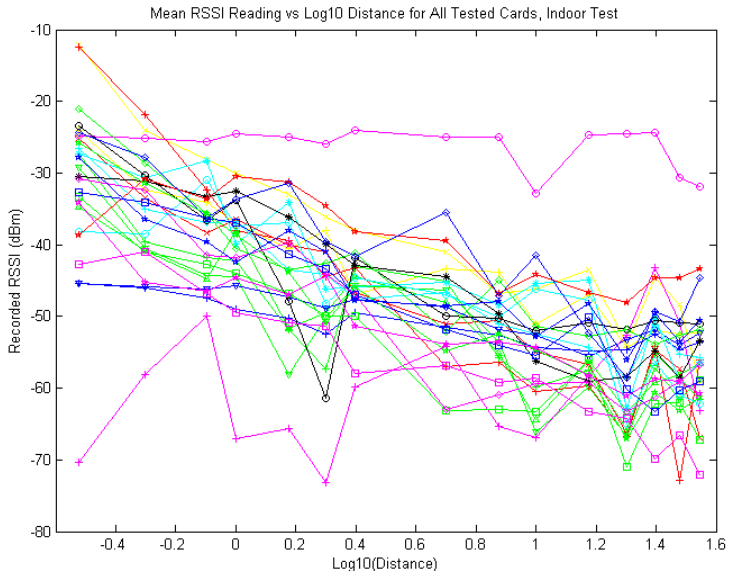
\includegraphics[width=\textwidth]{images/luiRSSI.png}
  \caption{Gemessener RSSI mit verschiedenen Access Points und Distanzen, aus \cite{lui2011differences}.}
  \label{fig:luiRSSI}
\end{figure}




\subsection{Verwandte Arbeiten - Fernlokalisierung \& indirekte Selbstlokalisierung mit 802.11}
Für die Fernlokalisierung mit 802.11 werden auf den Basisstationen Messwerte für empfangene Pakete bestimmt und daraus die Position der mobilen Einheit berechnet.
Diese Information kann anschließend an die mobile Einheit übertragen werden, dann handelt es sich um eine indirekte Selbstlokaliserung.

\subsubsection{RADAR}
\label{ch:Vorherige:sec:RADAR}
Das RADAR System von Bahl et al. (Microsoft Research) hat als eins der ersten WLAN-basierten Ortungssysteme viel Aufmerksamkeit erfahren \cite{bahl2000radar}.
Als Messgröße wird die Stärke des empfangenen Signals (received signal strength, RSS) genutzt, diese wird laut 802.11 Spezifikation als Index (RSSI) von der Hardware zurückgegeben. 
Das RADAR System ist auf eine offline-Phase angewiesen, in der empirisch ein Signalausbreitungsmodell aufgebaut wird. 
Es handelt sich also um ein System mit Szenenanalyse.\\
Die Verwendung einer offline-Phase ist im stark veränderlichen Baustellenumfeld nicht akzeptabel. 
Zum einen führt der ständige Baufortschritt dazu, dass regelmäßig neu kalibriert werden muss und zum anderen wirken sich auch die großen Baumaschinen auf die Signalausbreitung aus. 
Damit sich dies nicht im Modell wiederfindet, müssten zunächst alle beweglichen Maschinen aus dem Bereich entfernt werden, um anschließend in der online-Phase ihren Einfluss glätten zu können.
Die offline-Phase ist deshalb wirtschaftlich gesehen nicht durchführbar und das empirisch ermittelte Signalausbreitungsmodell müsste durch ein theoretisches ersetzt werden, für eine grobkörnige Bereichsortung sollte dies jedoch ausreichend sein.\\
Bei RADAR sendet die mobile Einheit vier UDP-Pakete pro Sekunde aus, an den Basisstationen wird dann der RSSI gemessen.
Die Autoren weisen jedoch darauf hin, dass sich dieser Vorgang leicht umkehren ließe, um von einer Fernlokalisierung auf eine Selbstlokalisierung zu kommen.
Bezüglich des Energieverbrauchs äußern sie sich jedoch zu keiner der beiden Varianten.\\
Die Position wird anschließend bestimmt, indem aus den in der offline-Phase aufgenommenen Werten derjenige mit dem geringsten Abstand zu den gemessen Werten gewählt wird. 
Dies wird im \textit{nearest neighbour in signal space (NNSS)} Algorithmus beschrieben.
Für die Ortung wird mehrfach gemessen und dann gemittelt, um im Median eine Genauigkeit von unter 3 Metern zu erhalten. 
Das kurze Sendeintervall von 0,25 Sekunden führt auch bei bewegten Personen zu einer Genauigkeit von 3,5 Metern.
Gleichzeitig sorgt das kurze Sendeintervall aber auch für einem hohen Energieverbrauch auf Seiten der mobilen Einheit, eine Reduktion der Sendevorgänge sollte im Kontext der Bereichsortung angestrebt werden, um den Energieverbrauch zu senken und die Batterielaufzeit der mobilen Einheit zu steigern.

\subsubsection{Verbesserungen an RADAR}
Bahl et al. veröffentlichten anschließend noch einige Verbesserungen für das ursprüngliche RADAR System \cite{bahl2000enhancements}.
Diese umfassen unter anderem den Einsatz von Access Points statt PCs als Basisstationen, verbesserte Ortung bewegter Personen und die Erkennung von hinzugekommenen Hindernissen wie etwa Personen.
Letzteres geschieht durch die Analyse der Signalstärke von Beacons anderer APs, da diese sich nicht bewegen, können Veränderungen in der Signalstärke als Veränderungen auf dem Signalweg gesehen werden.
Dies ließe sich auch auf größere Hindernisse übertragen, hängt aber stark von der strategischen Platzierung und möglichst dichten Verteilung der APs ab.\\
Auch hier äußern sich die Autoren nicht zum Energieverbrauch, wohl auch deshalb weil sie einen Laptop als mobile Einheit verwenden.

\subsubsection{Time-of-flight Lokalisierung}
\label{ch:Vorherige:sec:TOF}
Aufgrund der Schwächen von RSS-basierten Systemen wurde auch über solche nachgedacht, die stattdessen oder zusätzlich die time-of-flight (TOF) messen. 
Ein Beispiel für ein solches zeigen Wibowo et al. \cite{wibowo2009time}. 
Sie fordern optimalerweise Zugriff auf die physische Schicht (PHY) des 802.11 Protokolls, da auf diesen aber üblicherweise kein Zugriff besteht, messen sie TOF in der darüber liegenden MAC-Schicht.\\
Eine Basisstation sendet einen Beacon aus und protokolliert die Sendezeit, die mobile Einheit empfängt den Beacon, protokolliert die Empfangszeit und die Sendezeit der gesendeten Antwort, die Basisstation sichert die Empfangszeit der Antwort.
Nun sendet die mobile Einheit die zwei gespeicherten Zeitstempel an die Basisstation, der mit diesen die Verarbeitungszeit auf der mobilen Einheit berechnen kann, um dann die Distanz $d = c * (\frac{t_{empfangen} - t_{gesendet} - t_{Verarbeitung}}{2})$ zur mobilen Einheit zu bestimmen.
Dieses Schema lässt sich leicht von einer Fernlokalisierung in eine Selbstlokalisierung umwandeln, indem man den Initiator des Vorgangs tauscht.\\
Die Notwendigkeit die Zeitstempel bereits in der PHY- beziehungsweise MAC-Schicht zu setzen erfordert Zugriff auf die Software des als Basisstation verwendeten Access Points. 
Außerdem müssen die Zeitstempel im Bereich von Nanosekunden gesetzt werden und die Verarbeitungszeit vor/nach dem Setzen muss sehr konstant sein, da eine Abweichung von 100 ns bei c = 299.792.458 m/s bereits einen Fehler von 30 Metern verursacht.\\
Muthukrishnan et al. beschreiben diese Problematik bei dem Versuch TOF ohne Zugriff auf die Software des APs umzusetzen \cite{muthukrishnan2006using}.
Sie kommen zu dem Ergebnis, dass sich die in der Spezifikation eingebauten Zeitstempelfunktionen wie das Network Time Protocol (NTP), Ping und die Zeitstempel in Beacons nicht eignen, da sie zum einen nur eine Auflösung im Millisekundenbereich bieten und zum anderen von der Blockierungskontrolle von 802.11 (CSMA/CA) abhängen.

\subsubsection{Ortung ohne mobile Einheit}
Eine Ortung ohne mobile Einheit erfüllt wegen ihrer Abwesenheit offensichtlich jede Anforderung an die Batterielaufzeit der mobilen Einheit.
Mit MonoPHY stellen Abdel-Nasser et al. ein System zur Ortung ohne mobile Einheit vor \cite{abdel2013monophy}. \\
Dazu verwenden sie einen 802.11n-fähigen Laptop und Access Point und analysieren die Channel State Information (CSI) der physischen Schicht (PHY) der zwischen AP und Laptop übertragenen Daten.
Um die bestehende Struktur von APs zu nutzen, sollte das System angepasst und die CSI zwischen den APs gemessen werden.
Es hat jedoch einige Aspekte, die es ungeeignet für die Aufgabenstellung machen.\\
Das System unterscheidet nicht zwischen Personen, sondern erkennt nur, dass jemand anwesend ist. 
Außerdem ist es nur für eine Person in einem 100 $m^2$ Apartment gestaltet worden und müsste auf Baustellengröße und die Verfolgung vieler Personen erweitert werden.
Aber auch dann ist fraglich, wie gesichert werden kann, dass alle Personen durchgehend erkannt werden können, zum Beispiel wenn sich mehrere Personen auf oder in einem Transportfahrzeug aufhalten.
Auch ist es ohne Identifikation schwerer Fehler zu erkennen. 
Wird fälschlicherweise angezeigt, dass sich noch eine Peron im Tunnel befindet, kann oft durch ausrufen des Betreffenden festgestellt werden, dass dieser nicht im Tunnel ist. 
Hat man dagegen nur die Information, dass sich noch eine Person im Tunnel befindet, hat man keine Möglichkeit schnell herauszufinden ob dies der Wahrheit entspricht.\\
Weitere Probleme entstehen durch die Baumaschinen und Container. 
Diese haben einen starken Einfluss auf die CSI und verdecken dadurch möglicherweise nahe Personen und die Fahrzeugführer.
Deshalb müssten diese Objekte ebenfalls als Entitäten angezeigt werden. 
Die Anzeige diverser Kommandostände, Pausenräume und stehen gelassener Baumaschinen verwirrt im Notfall jedoch, da sich in jedem Objekt potentiell eine Person befinden könnte.\\
Die Veröffentlichung beruht außerdem auf der Verfügbarkeit der CSI, diese sind dort durch die Auswahl einer bestimmten Netzwerkkarte gegeben und sind nicht zwingend in einer bestehenden Struktur von APs verfügbar.
Als letzter Kritikpunkt steht die Verwendung eine offline-Phase, die, wie bereits diskutiert, wirtschaftlich nicht umsetzbar ist. \\ 
Somit erfüllt die Ortung ohne mobile Einheit zwar die Anforderungen an den Energieverbrauch, jedoch nicht die Forderung nach sicherer Erkennung von Abschnittswechseln, deshalb scheidet diese Technik zumindestens für Baustellen aus.




\subsection{Verwandte Arbeiten - Funkbasierte Lokalisierung ohne 802.11}
Die Arbeiten in dieser Kategorie verwenden nicht 802.11 für die Lokalisierung.
Sie verwenden stattdessen andere Protokolle, die sich durch einen geringeren Energieverbrauch als 802.11 auszeichnen sollen.

\subsubsection{Geeignete Messwerte für Bluetooth}
Hossain et al. untersuchen die laut Bluetooth Spezifikation zurückgegebenen Messwerte bezüglich ihrer Eignung für die Lokalisierung \cite{hossain2007comprehensive}.\\ 
Link Quality (LQ) beschreibt, wie gut die Verbindung zwischen zwei Geräten ist.
Der Wert wird aus der Bitfehlerrate beim Empfänger berechnet, allerdings ist nicht spezifiziert, wie der Wert zu berechnen ist, er hängt also in hohem Maße vom Hersteller des Empfängers ab. \\
Der Received Signal Strength Indicator (RSSI) misst die Stärke des eingehenden Signals, die Spezifikation sieht jedoch eine Golden Receive Power Range (GRPR) vor. 
Liegt der RSSI über oder unter dieser wird eine Anfrage zum erhöhen oder verringern der Sendeleistung an das andere Gerät verschickt, dies dient während einer aktiven Verbindung dazu den Energieverbrauch zu senken.
Problematisch am RSSI ist, dass er relativ zur GRPR bestimmt wird.
In der Untersuchung von Hossain et al. führte das dazu, dass der RSSI mit 0 gemessen wurde, wenn er innerhalb der GRPR lag. \\
Transmission Power Level (TPL) ist die Sendeleistung eines Geräts. 
TPL kann während einer bestehenden Verbindung durch Anfragen des Verbindungspartners verändert werden.
Dazu muss diese Energiesparfunktion jedoch unterstützt werden, was bei dem von Hossain et al. verwendeten Gerät nicht der Fall war.
Abbildung \ref{fig:bluetoothmess} zeigt deshalb für TPL eine waagerechte Linie.\\
Für Inquirys wird die Stärke des eingehenden Signals ohne die Beachtung des GRPR bestimmt.
Außerdem werden Inquirys immer mit voller Sendeleistung gesendet, da sie zur Entdeckung von Ressourcen verwendet werden.
Es handelt sich ebenfalls um den RSSI, um jedoch den Unterschied zum RSSI für eine Verbindung deutlich zu machen nennen Hossain et al. diesen Wert RX Power Level.

\begin{figure}[h]
  \centering
	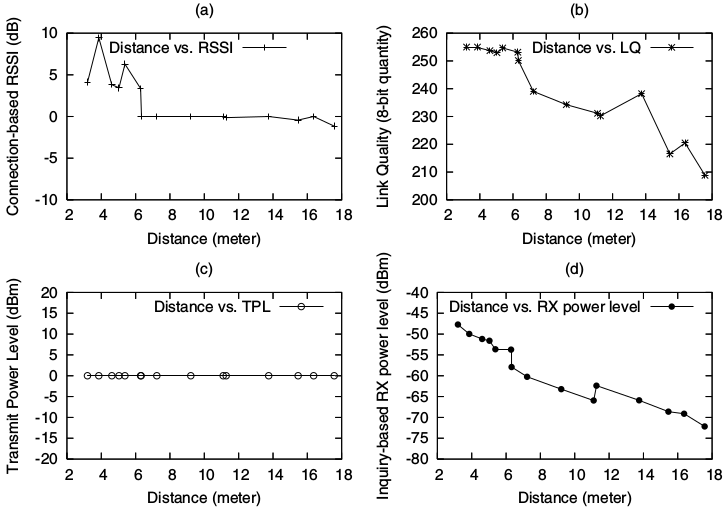
\includegraphics[width=\textwidth]{images/bluetoothmess.png}
  \caption{Korrelation der Messwerte mit der Distanz, aus \cite{hossain2007comprehensive}}
  \label{fig:bluetoothmess}
\end{figure}

\subsubsection{Antwortbasierte Inquiry Lokalisierung}
Bargh et al. stellen ein System zur Fernlokalisierung mittels Bluetooth Inquiry Scan vor \cite{bargh2008indoor}.
Die mobilen Einheiten sind dabei im discoverable ("{}entdeckbar"{}) Modus.
Die Basisstationen senden regelmäßig eine Inquiry Message aus, die dann von mobilen Einheiten in Reichweite mit einer Inquiry Response beantwortet werden. 
Anschließend werden die Antworten auf einem zentralen Ortungsserver gesammelt und die Positionen der mobilen Einheiten bestimmt.
Diese Information wird aus den beantworteten Inquiry Messages jeder mobilen Einheit gewonnen.
Dazu werden vorher in einer offline-Phase Fingerabdrücke für jeden Raum gesammelt.
In diesen wird gespeichert welche Inquiry Messages von der mobilen Einheit an einem bestimmten Ort beantwortet wurden.
Für die Bereichsortung entfiele diese offline-Phase, da der Bereich über die Beantwortung einer einzelnen Inquiry Message implizit bestimmt werden kann.
Tabelle \ref{table:irr} zeigt die abnehmende Warscheinlichkeit für eine Antwort auf die Inquiry Message mit steigender Distanz.

\begin{table}[h]
  \centering
  \caption{Rate der beantworteten Inquiry Messages (Inquiry Response Rate, IRR) gegen Distanz, aus \cite{bargh2008indoor}}
	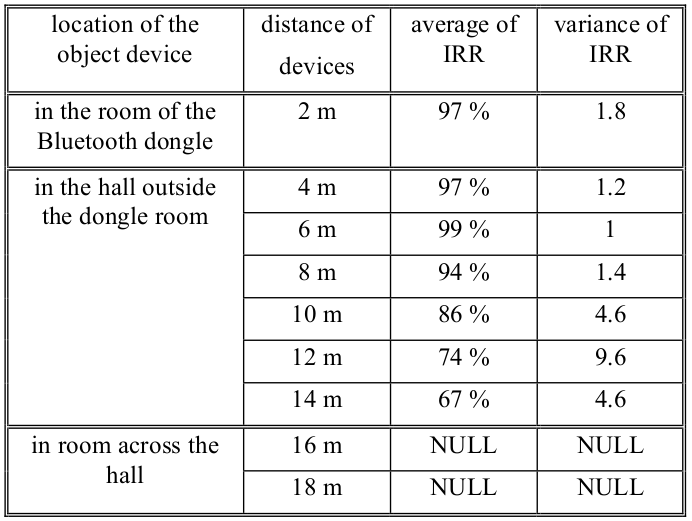
\includegraphics[width=0.7\textwidth]{images/irr.png}

  \label{table:irr}
\end{table}

\subsubsection{RSSI-basierte Inquiry Lokalisierung}
Ling et al. lokalisieren Bluetooth-fähige Geräte über den RSSI der Inquiry Response \cite{ling2010inquiry}.
Ihre Basisstationen versenden regelmäßig Inquiry Messages und messen den RSSI der Inquiry Responses.
Mobile Einheiten, die geortet werden wollen beziehungsweise sollen, bewerben in der Inquiry Response einen speziellen Service.
Dies erlaubt es diese herauszufiltern und die Privatsphäre anderer Personen zu wahren.
Die Autoren verwenden eine anfängliche offline-Phase um Fingerabdrücke für den RSSI an gegebenen zu finden.
Allerdings messen sie dazu an den Basisstationen die empfangene Signalstärke von Übertragungen anderer Basisstationen, folglich kann die offline-Phase automatisiert durchgeführt werden.
Für die online-Phase werden die gemessenen RSSI Werten über eine Warscheinlichkeitsverteilung geglättet, um eine bessere Ortungsgenauigkeit zu erreichen.
Für die eigentliche Lokalsierung werden die gemessenen RSSI mit den Warscheinlichkeitsverteilungen aus der offline-Phase verglichen und die Warscheinlichkeit für die Emission dieser Werte über die Position maximiert.

\subsubsection{RSSI-basierte BLE Lokalisierung}
Jianyong et al. stellen ein System zur Lokalisierung auf Basis von Bluetooth Low Energie (BLE, auch Bluetooth Smart) vor \cite{jianyong2014rssi}. \\
Sie messen an den Basisstationen den RSSI von Advertising Paketen, die zuvor von den mobilen Einheiten versendet wurden.
Für die genaue Ortung werden die Ergebnisse mit einem Gauß-Filter geglättet und für jede Basisstation die Parameter für ein Signalausbreitungsmodell bestimmt.
Die gemessene Signalstärke $P = A - 10n*log(d)$ hängt von der Referenzsignalstärke A im Abstand von einem Meter, dem Dämpfungsfaktor n und der Distanz d ab. \\
Jianyong et al. bestimmen die Referenzsignalstärke und den Dämpfungsfaktor für jede Basisstation.
Da jedoch nur eine Bereichsortung für diese Arbeit gefordert wurde, sollten A und n nur beispielhaft für eine Basisstation bestimmt werden, um den Aufwand beim Aufbau der Infrastruktur zu reduzieren.
Abbildung \ref{fig:blemodel} zeigt die von Jianyong et al. bestimmten Parameter für das Signalausbreitungsmodell. 
Abbildung \ref{fig:blemodel} zeigt außerdem, dass die verwendeten CC2540 Development Kit von Texas Instruments von einer Basisstation nur auf 20 Meter detektiert werden konnte.


\begin{figure}[h]
  \centering
	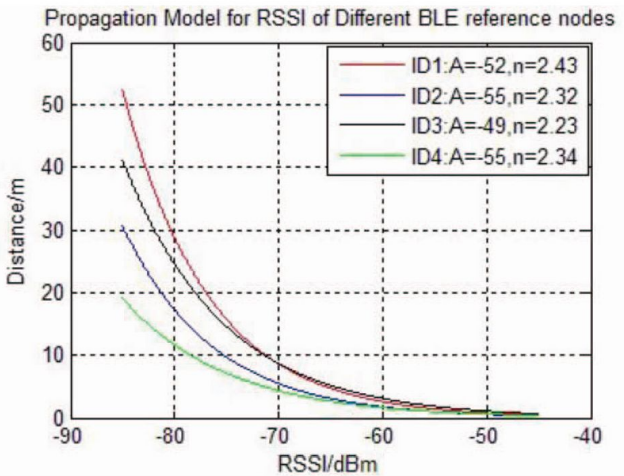
\includegraphics[width=0.7\textwidth]{images/blemodel.png}
  \caption{Signalausbreitungsmodelle aus \cite{jianyong2014rssi}}
  \label{fig:blemodel}
\end{figure}

\subsubsection{Lokalisierung mit LoRa}
Kim et al. stellen ein System zur Lokalisierung mit LoRa vor \cite{kim2016poster}.
Sie beziehen sich dabei auf eine Lokalisierung im Außenbereich in einem 30x30km Areal. 
Sie senden Pakete von der mobilen Einheit und messen die Time of Arrival (ToA) an den Basisstationen.
Dazu müssen die Basisstationen zeitsynchron arbeiten, dies wird über GPS sichergestellt.\\
Eine Lokalisierung über den RSSI lehnen sie ab, da dieser im Bereich von 20 bis 30km Entfernung nur um 3-6dBm fällt und die Varianz die Korrelation von RSSI und Distanz über lange Distanzen überdeckt.
Sie erreichen, abhängig von der Anzahl der verwendeten Basisstationen eien Genauigkeit zwischen wenigen Hundert und fast eintausend Metern, siehe dazu Abbildung \ref{fig:loraacc}

\begin{figure}[h]
  \centering
	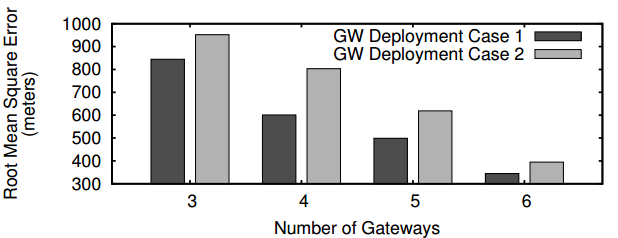
\includegraphics[width=0.7\textwidth]{images/loraacc.png}
  \caption{Quadratischer Fehler der Lokalisierung aus \cite{kim2016poster}, Gateways stellen Basisstationen dar.}
  \label{fig:loraacc}
\end{figure}


\section{Auswahl der Topologie}
Das Wissen um die Position der Nutzer soll nach der Ortung dem Sicherheitssystem der Baustelle zur Verfügung stehen. 
Das Sicherheitssystem fungiert daher konzeptionell auch als zentraler Ortungsserver.
Es muss deshalb eine Fernlokalisierung durchgeführt werden, diese kann aber sowohl direkt als auch indirekt durchgeführt werden. \\
Weil laut 802.11 keine für die Lokalisierung geeigneten Messwerte vom AP in das angeschlossene Netzwerk propagiert werden, kommt keine der verwandten Arbeiten zur direkten Fernlokalisierung ohne Zugriff auf die Software des AP aus.
In Abschnitt \ref{ch:Einleitung:sec:Zielsetzung} wurden sowohl Systeme ohne Änderungen der AP-Software als auch mit Änderungen dieser gefordert. \\
Diese Forderung lässt sich also in ein System zur indirekten Fernlokalisierung ohne Änderungen am AP und in ein System zur direkten Fernlokalisierung übersetzen.
Das System zur direkten Fernlokalisierung bedingt dabei Änderungen an der Software des AP, damit dieser den gewählten Messwert an den zentralen Ortungsserver übermittelt.\\
Dürfen Veränderungen der Hardware vorgenommen werden, bietet sich ebenfalls eine direkte Fernlokalisierung an, da dort die mobilen Einheiten, abgesehen von der Kollisionsdetektion/-vermeidung, nicht empfangen müssen.\\
Eine Topologie ohne Basisstationen kommt nicht in Frage, da diese Topologie Einzelpersonen insbesondere in Notsituationen nicht ausreichend gut erfasst.

\section{Auswahl des Funkprotokolls}
Soll das bestehende WLAN Netzwerk genutzt werden ist die Wahl auf die 802.11 Spezifikation beschränkt.\\
Für den dritten Schritt, der eine Änderung der verwendeten Hardware für die Basisstationen erlaubt, kann das Protokoll jedoch frei gewählt werden.
Bluetooth Low Energy wird gegenüber normalem Bluetooth aufgrund seiner Charakteristik als Protokoll für geringen Energieverbrauch bevorzugt.\\
LoRa bietet zwar theoretisch eine sehr hohe Reichweite, diese ist jedoch stark von verwendeten Antennen und den Hindernissen abhängig.
Ob LoRa einen signifikanten Vorteil bei der Reichweite hat muss geprüft werden.
Sollte dieser Vorteil bestehen, bietet LoRa durch seine bessere Abdeckung eine höhere Sicherheit bei der Erkennung von Abschnittswechseln. 
Außerdem ist es dadurch potentiell möglich auf triangulierte Positionen zu wechseln ohne mehr Basisstationen aufbauen zu müssen.


\section{Auswahl der Messwerte}
Da nur eine Bereichsortung durchgeführt werden soll, sind die Anforderungen an die Genauigkeit eines Messwertes gering.
Stattdessen sollte darauf geachtet werden, dass die Anforderung für die Messung gering ist.
Messwerte, die Zeitsynchronität vorraussetzen sind daher nicht geeignet.\\
Als Messwert wird der Received Signal Strength Index sowohl für WLAN als auch für Bluetooth Low Energy gewählt, da dieser bei jedem empfangenen Paket von der physischen Schicht gemessen und am empfangenden Gerät leicht ausgelesen werden kann.\\
Auch bei LoRa wird der RSSI gewählt. 
Da sich das Szenario im Gegensatz zu dem aus der Veröffentlichung von Kim et al. unter Tage abspielt kann keine Synchronisierung über GPS gewährleistet werden. 
Außerdem müssen die Distanzen zwischen den Basisstationen geringer gewählt werden, da die Ungenauigkeiten aus dieser Veröffentlichung zu hoch für das Szenario sind.
     % Analyse
%% entwurf.tex
%% $Id: entwurf.tex 61 2012-05-03 13:58:03Z bless $
%%

\chapter{Entwurf}
\label{ch:Entwurf}
%% ==============================
In diesem Kapitel erfolgt die ausf�hrliche Beschreibung des eigenen
L�sungsansatzes. Dabei sollten L�sungsalternativen diskutiert und
Entwurfsentscheidungen dargelegt werden.


Bla fasel\ldots

%% ==============================
\section{Abschnitt 1}
%% ==============================
\label{ch:Entwurf:sec:Abschnitt1}

Bla fasel\ldots

%% ==============================
\section{Abschnitt 2}
%% ==============================
\label{ch:Entwurf:sec:Abschnitt2}

Bla fasel\ldots

Blindtext Blindtext Blindtext Blindtext Blindtext Blindtext Blindtext
Blindtext Blindtext Blindtext Blindtext Blindtext Blindtext Blindtext
Blindtext Blindtext Blindtext Blindtext Blindtext Blindtext Blindtext
Blindtext Blindtext Blindtext Blindtext Blindtext Blindtext Blindtext
Blindtext Blindtext Blindtext Blindtext Blindtext Blindtext Blindtext
Blindtext Blindtext Blindtext Blindtext Blindtext Blindtext Blindtext
Blindtext Blindtext Blindtext Blindtext Blindtext Blindtext Blindtext
Blindtext Blindtext Blindtext Blindtext Blindtext Blindtext Blindtext
Blindtext Blindtext Blindtext Blindtext Blindtext Blindtext Blindtext
Blindtext Blindtext Blindtext Blindtext Blindtext Blindtext Blindtext
Blindtext Blindtext Blindtext Blindtext Blindtext Blindtext Blindtext
Blindtext Blindtext Blindtext Blindtext Blindtext Blindtext Blindtext
Blindtext Blindtext Blindtext Blindtext Blindtext Blindtext Blindtext
Blindtext Blindtext Blindtext Blindtext Blindtext Blindtext Blindtext
Blindtext Blindtext Blindtext Blindtext Blindtext Blindtext Blindtext
Blindtext Blindtext Blindtext Blindtext Blindtext Blindtext Blindtext
Blindtext Blindtext Blindtext Blindtext Blindtext Blindtext Blindtext

Blindtext Blindtext Blindtext Blindtext Blindtext Blindtext Blindtext
Blindtext Blindtext Blindtext Blindtext Blindtext Blindtext Blindtext
Blindtext Blindtext Blindtext Blindtext Blindtext Blindtext Blindtext
Blindtext Blindtext Blindtext Blindtext Blindtext Blindtext Blindtext
Blindtext Blindtext Blindtext Blindtext Blindtext Blindtext Blindtext
Blindtext Blindtext Blindtext Blindtext Blindtext Blindtext Blindtext
Blindtext Blindtext Blindtext Blindtext Blindtext Blindtext Blindtext
Blindtext Blindtext Blindtext Blindtext Blindtext Blindtext Blindtext
Blindtext Blindtext Blindtext Blindtext Blindtext Blindtext Blindtext
Blindtext Blindtext Blindtext Blindtext Blindtext Blindtext Blindtext
Blindtext Blindtext Blindtext Blindtext Blindtext Blindtext Blindtext
Blindtext Blindtext Blindtext Blindtext Blindtext Blindtext Blindtext
Blindtext Blindtext Blindtext Blindtext Blindtext Blindtext Blindtext
Blindtext Blindtext Blindtext Blindtext Blindtext Blindtext Blindtext
Blindtext Blindtext Blindtext Blindtext Blindtext Blindtext Blindtext
Blindtext Blindtext Blindtext Blindtext Blindtext Blindtext Blindtext
Blindtext Blindtext Blindtext Blindtext Blindtext Blindtext Blindtext
Blindtext Blindtext Blindtext Blindtext Blindtext Blindtext Blindtext
Blindtext Blindtext Blindtext Blindtext Blindtext Blindtext Blindtext
Blindtext Blindtext Blindtext Blindtext Blindtext Blindtext Blindtext

Blindtext Blindtext Blindtext Blindtext Blindtext Blindtext Blindtext
Blindtext Blindtext Blindtext Blindtext Blindtext Blindtext Blindtext
Blindtext Blindtext Blindtext Blindtext Blindtext Blindtext Blindtext
Blindtext Blindtext Blindtext Blindtext Blindtext Blindtext Blindtext
Blindtext Blindtext Blindtext Blindtext Blindtext Blindtext Blindtext
Blindtext Blindtext Blindtext Blindtext Blindtext Blindtext Blindtext
Blindtext Blindtext Blindtext Blindtext Blindtext Blindtext Blindtext
Blindtext Blindtext Blindtext Blindtext Blindtext Blindtext Blindtext
Blindtext Blindtext Blindtext Blindtext Blindtext Blindtext Blindtext
Blindtext Blindtext Blindtext Blindtext Blindtext Blindtext Blindtext
Blindtext Blindtext Blindtext Blindtext Blindtext Blindtext Blindtext
Blindtext Blindtext Blindtext Blindtext Blindtext Blindtext Blindtext
Blindtext Blindtext Blindtext Blindtext Blindtext Blindtext Blindtext
Blindtext Blindtext Blindtext Blindtext Blindtext Blindtext Blindtext
Blindtext Blindtext Blindtext Blindtext Blindtext Blindtext Blindtext

Blindtext Blindtext Blindtext Blindtext Blindtext Blindtext Blindtext
Blindtext Blindtext Blindtext Blindtext Blindtext Blindtext Blindtext
Blindtext Blindtext Blindtext Blindtext Blindtext Blindtext Blindtext
Blindtext Blindtext Blindtext Blindtext Blindtext Blindtext Blindtext
Blindtext Blindtext Blindtext Blindtext Blindtext Blindtext Blindtext
Blindtext Blindtext Blindtext Blindtext Blindtext Blindtext Blindtext
Blindtext Blindtext Blindtext Blindtext Blindtext Blindtext Blindtext
Blindtext Blindtext Blindtext Blindtext Blindtext Blindtext Blindtext
Blindtext Blindtext Blindtext Blindtext Blindtext Blindtext Blindtext
Blindtext Blindtext Blindtext Blindtext Blindtext Blindtext Blindtext
Blindtext Blindtext Blindtext Blindtext Blindtext Blindtext Blindtext
Blindtext Blindtext Blindtext Blindtext Blindtext Blindtext Blindtext
Blindtext Blindtext Blindtext Blindtext Blindtext Blindtext Blindtext
Blindtext Blindtext Blindtext Blindtext Blindtext Blindtext Blindtext
Blindtext Blindtext Blindtext Blindtext Blindtext Blindtext Blindtext
Blindtext Blindtext Blindtext Blindtext Blindtext Blindtext Blindtext

Blindtext Blindtext Blindtext Blindtext Blindtext Blindtext Blindtext
Blindtext Blindtext Blindtext Blindtext Blindtext Blindtext Blindtext
Blindtext Blindtext Blindtext Blindtext Blindtext Blindtext Blindtext
Blindtext Blindtext Blindtext Blindtext Blindtext Blindtext Blindtext
Blindtext Blindtext Blindtext Blindtext Blindtext Blindtext Blindtext
Blindtext Blindtext Blindtext Blindtext Blindtext Blindtext Blindtext
Blindtext Blindtext Blindtext Blindtext Blindtext Blindtext Blindtext
Blindtext Blindtext Blindtext Blindtext Blindtext Blindtext Blindtext
Blindtext Blindtext Blindtext Blindtext Blindtext Blindtext Blindtext
Blindtext Blindtext Blindtext Blindtext Blindtext Blindtext Blindtext
Blindtext Blindtext Blindtext Blindtext Blindtext Blindtext Blindtext
Blindtext Blindtext Blindtext Blindtext Blindtext Blindtext Blindtext
Blindtext Blindtext Blindtext Blindtext Blindtext Blindtext Blindtext

%% ==============================
\section{Zusammenfassung}
%% ==============================
\label{ch:Entwurf:sec:zusammenfassung}

Am Ende sollten ggf. die wichtigsten Ergebnisse nochmal in \emph{einem}
kurzen Absatz zusammengefasst werden.

%%% Local Variables: 
%%% mode: latex
%%% TeX-master: "thesis"
%%% End: 
     % Entwurf
%% implemen.tex
%% $Id: implemen.tex 61 2012-05-03 13:58:03Z bless $
%%

\chapter{Implementierung}
\label{ch:Implementierung}
%% ==============================
Bla fasel\ldots

%% ==============================
\section{Abschnitt 1}
%% ==============================
\label{ch:Implementierung:sec:Abschnitt1}

Bla fasel\ldots

%% ==============================
\section{Abschnitt 2}
%% ==============================
\label{ch:Implementierung:sec:Abschnitt2}

Bla fasel\ldots

%%% Local Variables: 
%%% mode: latex
%%% TeX-master: "thesis"
%%% End: 
    % Implementierung
%% eval.tex
%% $Id: eval.tex 61 2012-05-03 13:58:03Z bless $

\chapter{Evaluierung}
\label{ch:Evaluierung}
%% ==============================
Hier kommt der Nachweis, dass das in Kapitel~\ref{ch:Entwurf}
entworfene Konzept auch funktioniert. Leistungsmessungen einer
Implementierung werden auch immer gerne gesehen.

Bla fasel\ldots

%% ==============================
\section{Abschnitt 1}
%% ==============================
\label{ch:Evaluierung:sec:Abschnitt1}

Bla fasel\ldots

%% ==============================
\section{Abschnitt 2}
%% ==============================
\label{ch:Evaluierung:sec:Abschnitt2}

Bla fasel\ldots

%% ==============================
\section{Zusammenfassung}
%% ==============================
\label{ch:Evaluierung:sec:zusammenfassung}

Am Ende sollten ggf. die wichtigsten Ergebnisse nochmal in \emph{einem}
kurzen Absatz zusammengefasst werden.

%%% Local Variables: 
%%% mode: latex
%%% TeX-master: "thesis"
%%% End: 
        % Evaluierung
%% zusammenf.tex
%% $Id: zusammenf.tex 61 2012-05-03 13:58:03Z bless $
%%

\chapter{Zusammenfassung und Ausblick}
\label{ch:Zusammenfassung}
%% ==============================
Bla fasel\ldots

(Keine Untergliederung mehr!)

%%% Local Variables: 
%%% mode: latex
%%% TeX-master: "thesis"
%%% End: 
   % Zusammenfassung und Ausblick

%% ++++++++++++++++++++++++++++++++++++++++++
%% Anhang
%% ++++++++++++++++++++++++++++++++++++++++++

\appendix
%\include{anhang_a}
%\include{anhang_b}

%% ++++++++++++++++++++++++++++++++++++++++++
%% Literatur
%% ++++++++++++++++++++++++++++++++++++++++++
%  mit dem Befehl \nocite werden auch nicht 
%  zitierte Referenzen abgedruckt
\cleardoublepage
\phantomsection
\addcontentsline{toc}{chapter}{\bibname}
%%
\nocite{*} % nur angeben, wenn auch nicht im Text zitierte Quellen 
           % erscheinen sollen
\bibliographystyle{itmabbrv} % mit abgekürzten Vornamen der Autoren
%\bibliographystyle{gerplain} % abbrvnat unsrtnat
% spezielle Zitierstile: Labels mit vier Buchstaben und Jahreszahl
%\bibliographystyle{itmalpha}  % ausgeschriebene Vornamen der Autoren
\bibliography{thesis}
%% ++++++++++++++++++++++++++++++++++++++++++
%% Index
%% ++++++++++++++++++++++++++++++++++++++++++
\ifnotdraft{
\cleardoublepage
\phantomsection
\printindex            % Index, Stichwortverzeichnis
}
\end{document}
%% end of file
